% Numerical evidence for Part II (source: results/RESULTS_PARADIGM.md; numbers checked against the
% per-experiment files results/*/table*.md and results/langevin_global/gibbs_reference.md).
\section{Numerical evidence}\label{sec:evidence}

Every number in this section is produced by the named script from raw files, and no table is edited by hand. The
scripts are in the directory \code{experiments/} of the accompanying repository and write their output to
subdirectories of \code{results/}; ``\code{script.py} $\to$ \code{dir/}'' below names a script and its output
directory or file.

\begin{itemize}
  \item The test files \code{tests/test_transport.py}, \code{tests/test_langevin.py} and \code{tests/test_averaging.py}
    check the inequalities at every sample of simulated trajectories, or on sampled states.
  \item They are run with \texttt{venv\textbackslash Scripts\textbackslash python -m pytest tests}. The current
    number of tests is given in the repository's \code{README.md}.
\end{itemize}

% ------------------------------------------------------------------------------------------------ B
\subsection{Theorem B: the label-free Lyapunov function}

Script: \code{exp_transport_permutation.py} $\to$ \code{transport_permutation/}.

Each network starts as a random relabelling of the ideal configuration plus noise $0.05$, with mean-field gains and
3 seeds per $m$. ``Excess'' is $\abs{(1/m)\sum\text{Taylor remainders}}$, the part that actually enters $\dot V$.
Table~\ref{tab:evidence:permutation} and Figure~\ref{fig:evidence:permutation} show the results.

\begin{table}[htbp]
\centering
\footnotesize
\caption{Theorem B, permuted-ideal start, mean-field gains; means over 3 seeds. The two bounds are the same bound,
evaluated with the matched (OT) error and with the labelled error, along the same trajectory.}
\label{tab:evidence:permutation}
\begin{tabularx}{\textwidth}{@{}c*{6}{Y}@{}}
\toprule
$m$ & labelled error ($t=0$) & OT error $W$ ($t=0$) & $\RMS\norm{e}$ & actual excess & bound, matched error
  & same bound, labelled error\\
\midrule
8  & 2.675 & 0.1070 & 0.0113 & $1.96\cdot10^{-5}$ & $8.27\cdot10^{-2}$ & 2.93\\
16 & 2.532 & 0.1044 & 0.0065 & $9.58\cdot10^{-6}$ & $4.37\cdot10^{-2}$ & 1.86\\
32 & 2.684 & 0.1122 & 0.0079 & $2.69\cdot10^{-5}$ & $7.07\cdot10^{-2}$ & 2.11\\
64 & 2.764 & 0.1136 & 0.0094 & $1.23\cdot10^{-5}$ & $6.80\cdot10^{-2}$ & 2.43\\
\bottomrule
\end{tabularx}
\end{table}

\begin{itemize}
  \item The bound is at least the actual excess at every sample of every run.
  \item The matched error is about $1/25$ of the labelled one.
  \item The bound is 30--45$\times$ smaller when evaluated with the matched error.
  \item Nothing grows with $m$.
  \item The bounds remain far above the actual excess, because the Hessian supremum is global.
\end{itemize}

\begin{figure}[htbp]
\centering
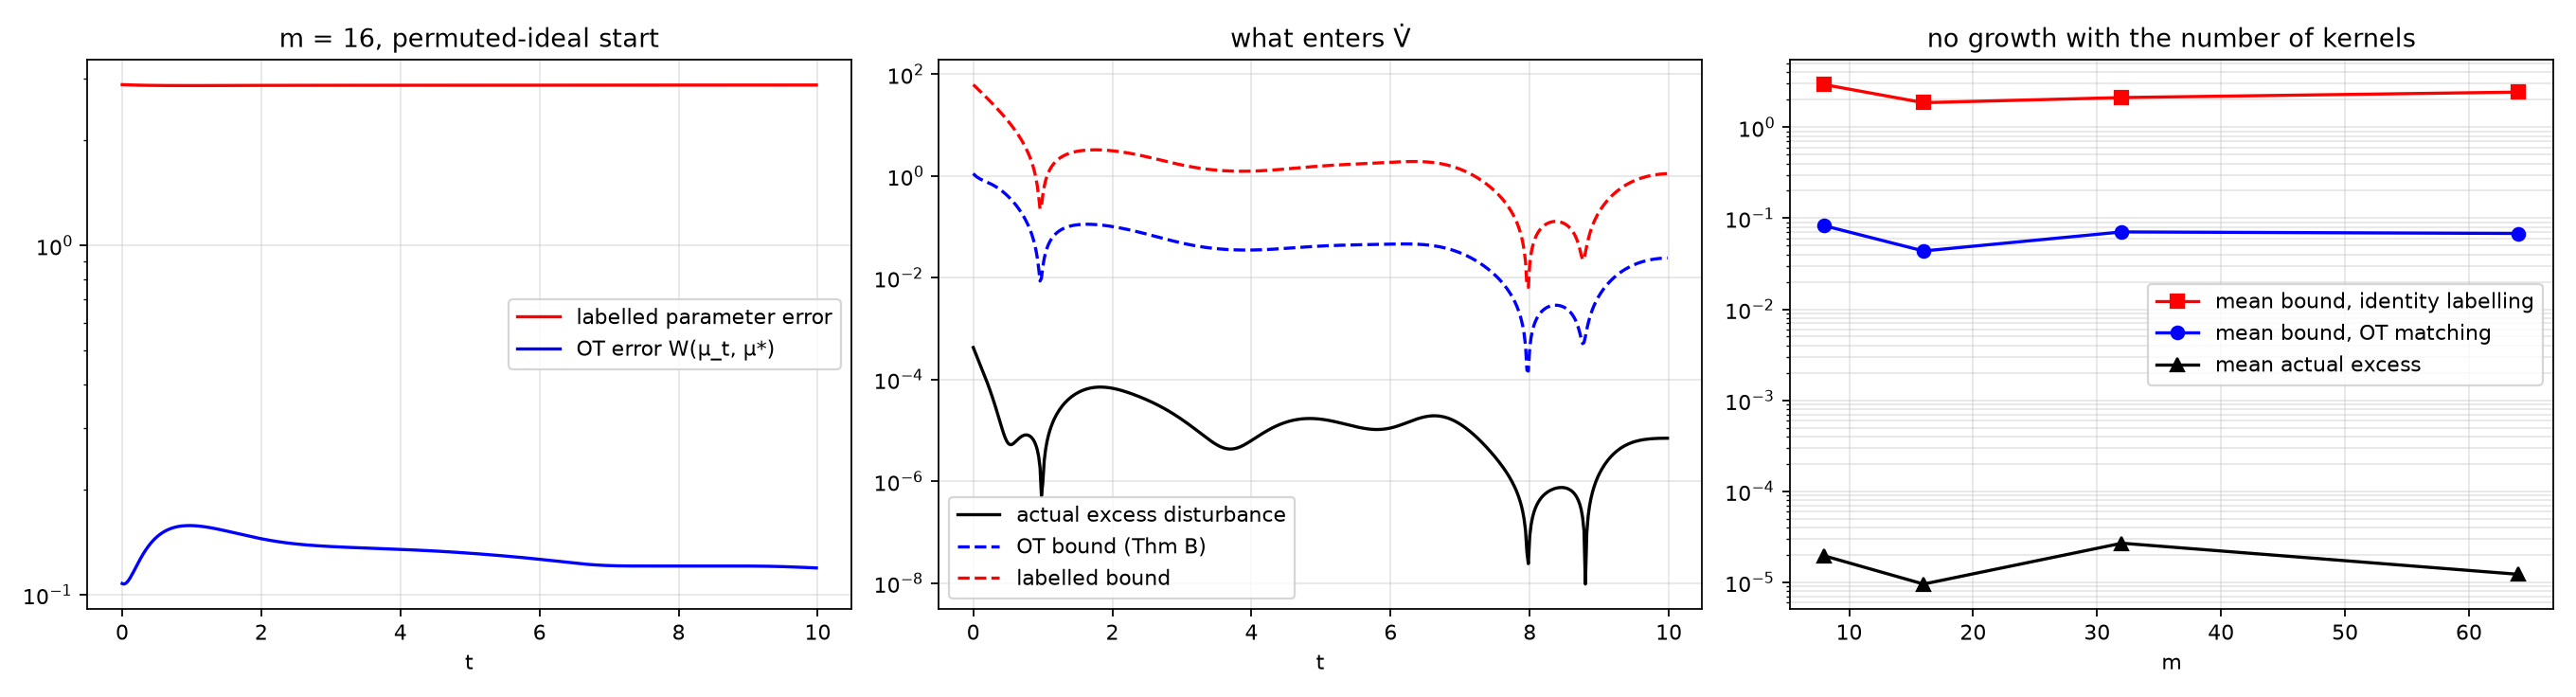
\includegraphics[width=0.95\textwidth]{transport_permutation/figure.png}
\caption{Theorem B, permuted-ideal start. Left: labelled parameter error and OT error $W(\mu_t,\mu^*)$ for $m=16$.
Centre: the actual excess disturbance that enters $\dot V$, the OT bound of Theorem B and the labelled bound, for
$m=16$. Right: the mean bound with identity labelling, the mean bound with OT matching and the mean actual excess,
against $m$.}
\label{fig:evidence:permutation}
\end{figure}

\paragraph{Corollary B.5 along \texorpdfstring{$\Lsig$}{(L-sigma)}.} This is checked by the test
\code{test_corollary_B5_fails_along_lsigma_and_its_leak_variant_holds}. The test asserts every hypothesis of C(iv) and
measures $\sup W\le\bar\eta$. There, the plain B.5 bound is exceeded by more than $3\times$, while the leak variant
with $\sigma_m b^2/4$ holds.

% ------------------------------------------------------------------------------------------------ C
\subsection{Theorem C: OT \texorpdfstring{$\sigma$}{sigma}-modification}

Scripts: \code{exp_ot_sigma_mod.py} and \code{exp_sigma_mod_transient.py} $\to$ \code{ot_sigma_mod/}.

The two starts share plant, prior, geometry and $x_0$. They differ only in particle labels
(Table~\ref{tab:evidence:sigmamod}, Figure~\ref{fig:evidence:sigmamod}). Table~\ref{tab:evidence:transient} shows
the reshuffling transient from the relabelled start (5 seeds).

\begin{table}[htbp]
\centering
\small
\caption{Theorem C: OT $\sigma$-modification against labelled $\sigma$-modification (oracle plant, $m=6$, 5 seeds,
$\sigma_m=0.3$). $\RMS\norm{e}$ is taken over $20$--$40$\,s and reported as mean $\pm$ 95\% confidence interval over seeds;
$W_{\mathrm{end}}$ is the OT error at the end.}
\label{tab:evidence:sigmamod}
\begin{tabular}{@{}llccc@{}}
\toprule
start & mechanism & $\RMS\norm{e}$ (20--40\,s) & $W_{\mathrm{end}}$ & labelled error at end\\
\midrule
aligned    & projection                 & $0.0051\pm0.0010$ & 0.2953 & 0.2953\\
aligned    & labelled $\sigma$-mod.     & $0.0091\pm0.0018$ & 0.3040 & 0.3040\\
aligned    & OT $\sigma$-mod.           & $0.0091\pm0.0018$ & 0.3040 & 0.3040\\
relabelled & projection                 & $0.0051\pm0.0010$ & 0.2953 & 0.2953\\
relabelled & labelled $\sigma$-mod.     & $0.0091\pm0.0018$ & 0.3040 & \textbf{2.0590}\\
relabelled & OT $\sigma$-mod.           & $0.0091\pm0.0018$ & 0.3040 & 0.3040\\
\bottomrule
\end{tabular}
\end{table}

\begin{table}[htbp]
\centering
\small
\caption{Reshuffling transient from the relabelled start ($m=6$, 5 seeds, $\sigma_m=0.3$): $\RMS\norm{e}$ over
time windows, and the particle path length.}
\label{tab:evidence:transient}
\begin{tabular}{@{}lccccc@{}}
\toprule
leak & $[0,5]$\,s & $[5,10]$\,s & $[10,20]$\,s & $[20,40]$\,s & particle path length\\
\midrule
labelled & 0.0771 & 0.0086 & 0.0093 & 0.0091 & 2.2585\\
OT       & 0.0743 & 0.0072 & 0.0093 & 0.0091 & 0.3917\\
\bottomrule
\end{tabular}
\end{table}

\begin{itemize}
  \item The labelled leak's longer path costs only about 4\% of early $\RMS\norm{e}$. Theorem F does not price
    leak-driven transport (Proposition C.5).
  \item The C(iv) instance in the tests satisfies every hypothesis, asserted. $\VOT$ stays below the envelope
    $e^{-\alpha t}V(0)+\beta/\alpha$ at every sample and contracts by more than $5\times$.
  \item The C(ii) test asserts $C\le b^2+4\eta R$, $\sqrt C\le b+2\eta$, and $C=b^2$ under both gap conditions, on
    300 configurations.
\end{itemize}

\begin{figure}[htbp]
\centering
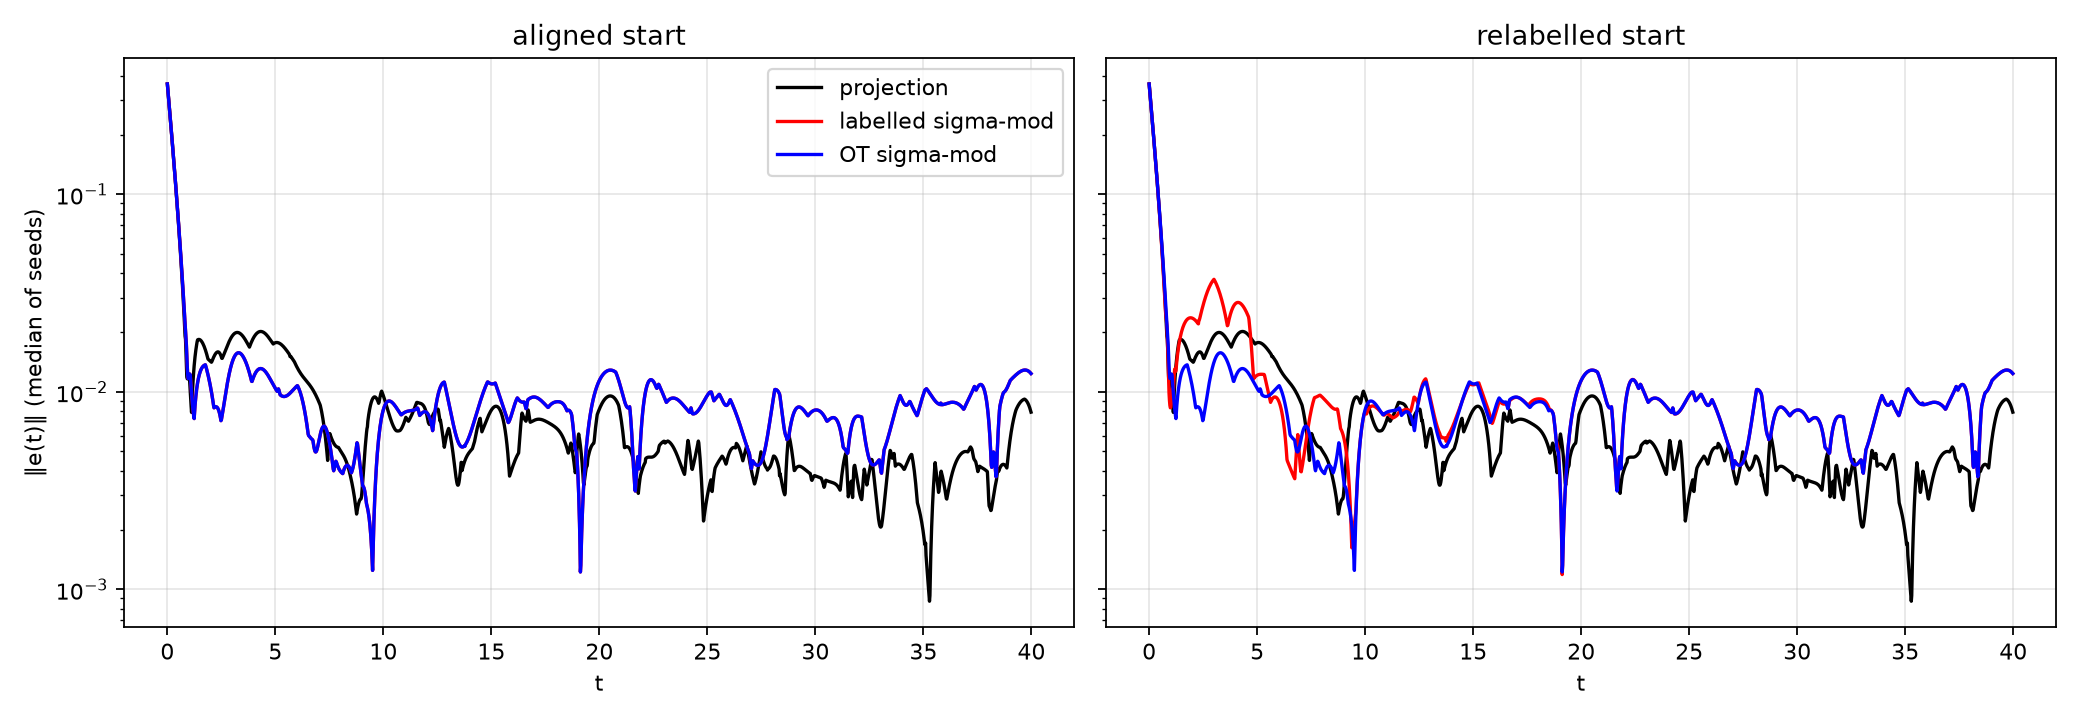
\includegraphics[width=0.9\textwidth]{ot_sigma_mod/figure.png}
\caption{Theorem C: $\norm{e(t)}$ (median of seeds) for projection, labelled $\sigma$-modification and OT
$\sigma$-modification, from the aligned start (left) and from the relabelled start (right).}
\label{fig:evidence:sigmamod}
\end{figure}

% ------------------------------------------------------------------------------------------------ D
\subsection{Theorem D: convergence in \texorpdfstring{$m$}{m}}

Script: \code{exp_mean_field_m.py} $\to$ \code{mean_field_m/}. Table~\ref{tab:evidence:meanfield} and
Figure~\ref{fig:evidence:meanfield} show the results.

\begin{table}[htbp]
\centering
\small
\caption{Theorem D: mean-field consistency in $m$ (Van der Pol plant, mean-field gains, smooth initial measure
quantised at $m$ points). The ratio is $W(\mu^m_T,\mu^{2m}_T)/W(\mu^m_0,\mu^{2m}_0)$.}
\label{tab:evidence:meanfield}
\begin{tabular}{@{}lcccc@{}}
\toprule
$m$ & $\sup_t\norm{e^m-e^{2m}}$ & $W(\mu^m_0,\mu^{2m}_0)$ & $W(\mu^m_T,\mu^{2m}_T)$ & ratio\\
\midrule
16 vs 32   & 0.0046 & 0.2179 & 0.3658 & 1.68\\
32 vs 64   & 0.0009 & 0.1091 & 0.1788 & 1.64\\
64 vs 128  & 0.0001 & 0.0545 & 0.0920 & 1.69\\
128 vs 256 & 0.0000 & 0.0273 & 0.0459 & 1.68\\
\bottomrule
\end{tabular}
\end{table}

This is a consistency check in $m$, not a check of the constant.
\begin{itemize}
  \item The guaranteed factor $e^{\Lambda T}$ is at least $e^{496}$ on this box.
  \item The Van der Pol plant fails the tube condition of Theorem D(b), so the run is covered by the localised D(d).
\end{itemize}

\begin{figure}[htbp]
\centering
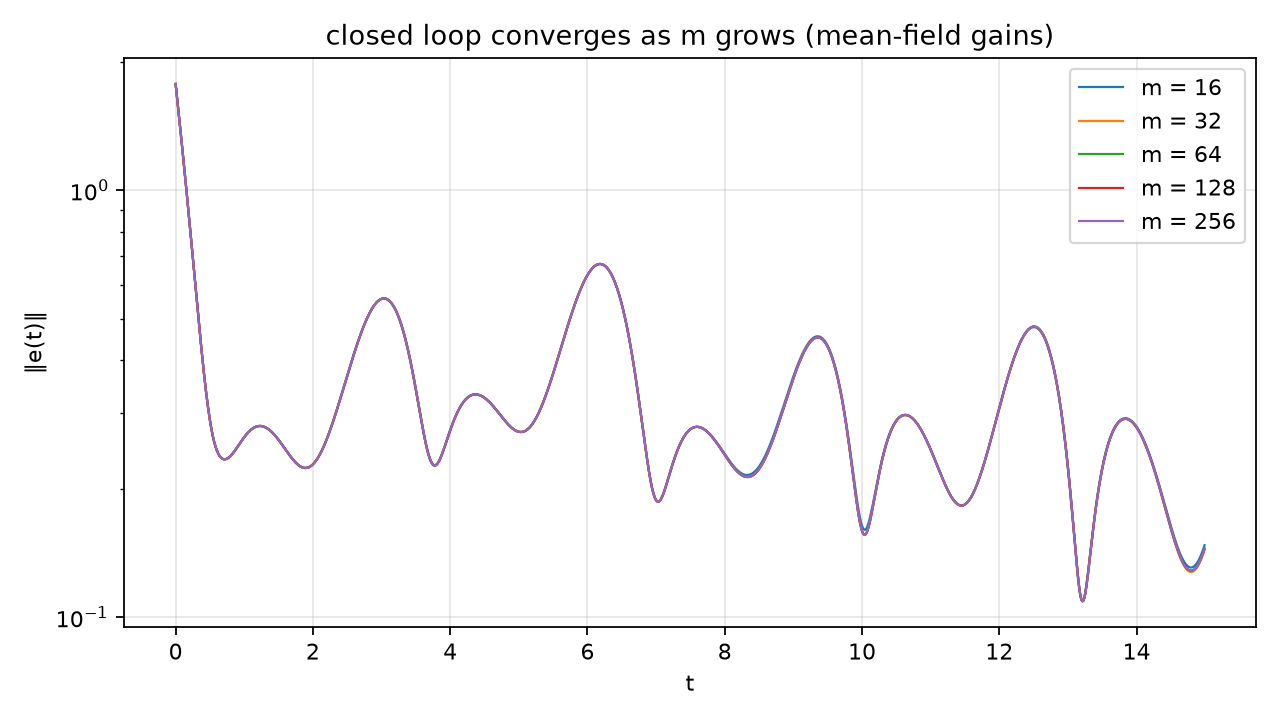
\includegraphics[width=0.8\textwidth]{mean_field_m/figure.png}
\caption{Theorem D: tracking error $\norm{e(t)}$ of the closed loop (Van der Pol plant, mean-field gains) for
$m=16$, $32$, $64$, $128$ and $256$.}
\label{fig:evidence:meanfield}
\end{figure}

% ------------------------------------------------------------------------------------------------ E
\subsection{Theorem E: label-free convergence under excitation}

Script: \code{exp_pe_convergence.py} $\to$ \code{pe_convergence/}. Table~\ref{tab:evidence:pe} and
Figure~\ref{fig:evidence:pe} show the results.

\begin{table}[htbp]
\centering
\footnotesize
\caption{Theorem E: tangential excitation and label-free parameter convergence ($m=3$, $n=2$, permuted start,
$T=200$\,s). $\lambda_{\min}$ is that of the excitation Gramian.}
\label{tab:evidence:pe}
\begin{tabularx}{\textwidth}{@{}lc*{5}{Y}@{}}
\toprule
reference & seed & $\lambda_{\min}$, first 60\,s window & min over sliding 60\,s windows & $W(T)/W(0)$
  & fitted rate of $W$, $t\ge100$\,s (1/s) & labelled$(T)$\,/ labelled$(0)$\\
\midrule
rich (6 tones) & 0 & $8.60\cdot10^{-3}$ & $4.12\cdot10^{-3}$ & 0.544 & $2.31\cdot10^{-3}$ & 0.992\\
rich (6 tones) & 1 & $5.52\cdot10^{-3}$ & $1.02\cdot10^{-3}$ & 0.409 & $2.32\cdot10^{-3}$ & 0.962\\
rich (6 tones) & 2 & $1.08\cdot10^{-3}$ & $5.91\cdot10^{-4}$ & 0.369 & $3.07\cdot10^{-3}$ & 1.007\\
single sine    & 0 & $2.54\cdot10^{-2}$ & $2.41\cdot10^{-2}$ & 0.274 & $4.05\cdot10^{-3}$ & 0.988\\
single sine    & 1 & $2.96\cdot10^{-2}$ & $2.71\cdot10^{-2}$ & 0.314 & $4.26\cdot10^{-3}$ & 0.967\\
single sine    & 2 & $6.74\cdot10^{-3}$ & $6.61\cdot10^{-3}$ & 0.226 & $2.91\cdot10^{-3}$ & 1.008\\
\bottomrule
\end{tabularx}
\end{table}

\begin{itemize}
  \item The matched error decays in all six runs. The labelled error stays within 4\% of its initial value.
  \item The rank correlation between the uniform excitation level and the fitted rate is 0.60 over the six runs. The
    PE level is a hypothesis of Theorem E, not a rate predictor (Remark E.1).
  \item The proof's linearisation is checked exactly: the Jacobian equals $A(t)$, and
    $QA+A^\T Q=\operatorname{diag}(-k_eI,0)$.
\end{itemize}

\begin{figure}[htbp]
\centering
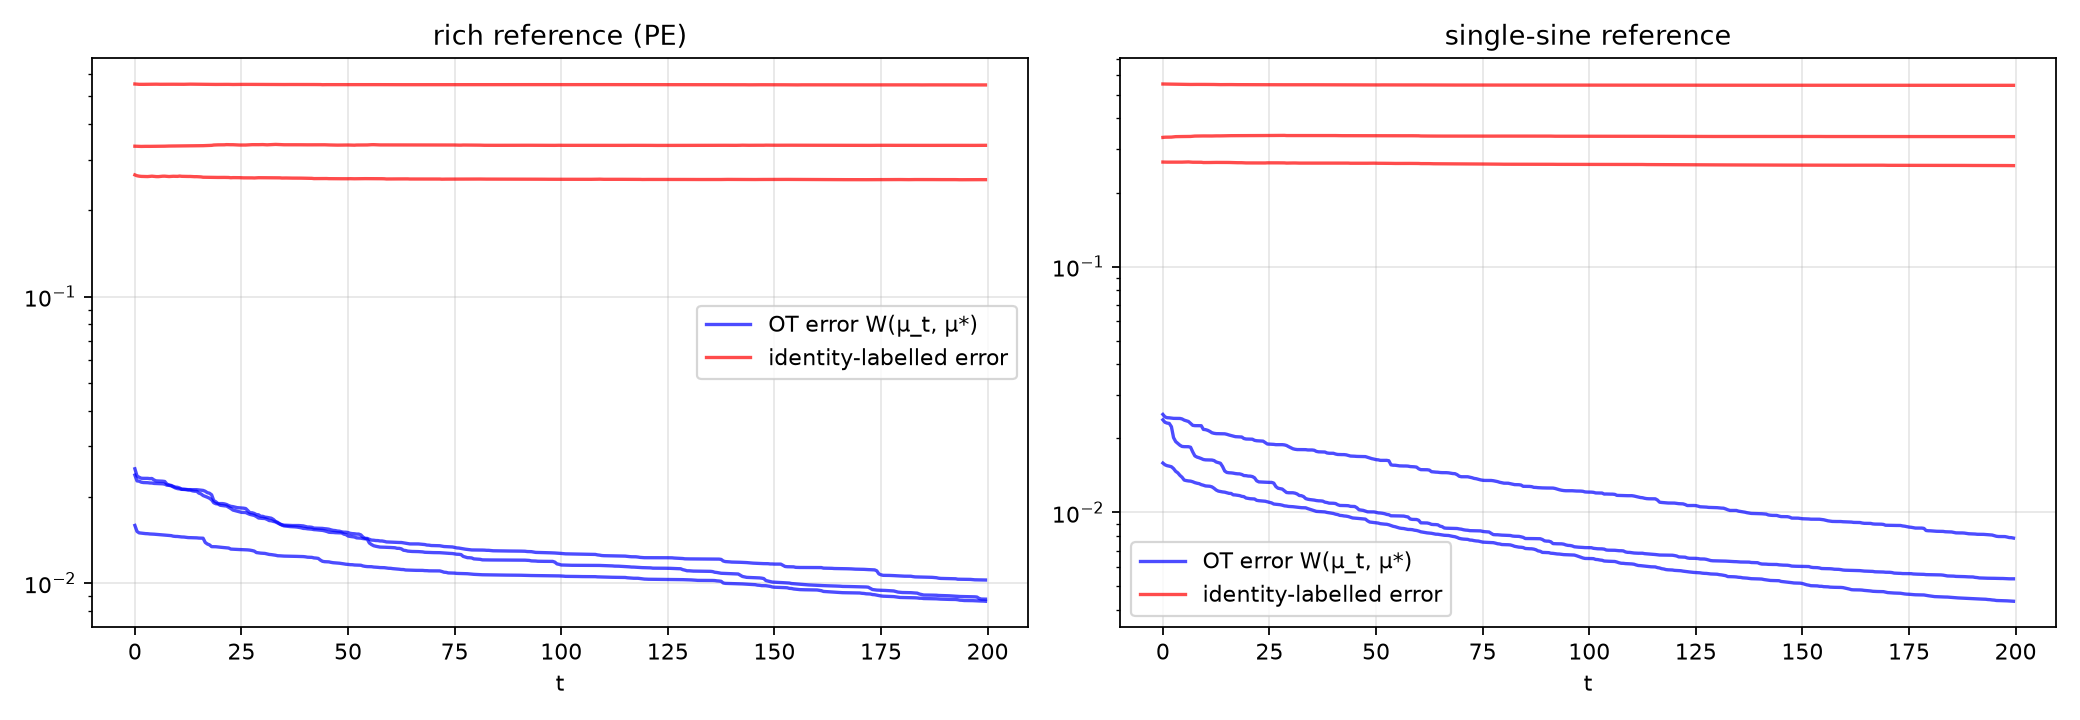
\includegraphics[width=0.9\textwidth]{pe_convergence/figure.png}
\caption{Theorem E: OT error $W(\mu_t,\mu^*)$ and identity-labelled error for the three seeds, with the rich
reference (left) and the single-sine reference (right).}
\label{fig:evidence:pe}
\end{figure}

% ------------------------------------------------------------------------------------------------ F
\subsection{Theorem F: transport cost}

Theorem F is checked by tests.
\begin{itemize}
  \item Along (L), the particle path length (which is at least the Wasserstein length) stays below
    $\lambda_G^{1/2}L_1\int\norm{e}$ at every sample.
  \item Along $\Lsig$ with the OT leak, $W(\mu_{t_1},\mu_{t_0})\le\int(\lambda_G^{1/2}L_1\norm{e}+\sigma_mW(\mu_r,\mu^0))$
    on a grid of pairs.
  \item Lemma P.1 holds on 2000 adversarial states, and a tight instance of F(i) reaches ratio $\ge0.99$.
\end{itemize}

% ------------------------------------------------------------------------------------------------ G
\subsection{Proposition G: slow geometry}

Scripts: \code{exp_variable_projection.py} and \code{exp_slow_manifold_slope.py}, both $\to$
\code{variable_projection/}.

In Table~\ref{tab:evidence:varpro}, ranges are along the run (5 samples), and ``$a$\,/\,$b$'' means
first-quarter\,/\,last-quarter medians. Velocities are centred differences of period means.

\begin{table}[htbp]
\centering
\small
\caption{Proposition G: the two configurations, \texttt{violating} ($m=4$, $k_e=20$, $g_a=2$, $\delta=0.1$,
$T=800$\,s) and \texttt{satisfying} ($m=2$, $k_e=20$, $g_a=13$, $\delta=0.004$, $T=3000$\,s). In the rows for $L^*$
and $\bar L$, ``$x\to y$'' is first sample $\to$ last sample.}
\label{tab:evidence:varpro}
\begin{tabularx}{\textwidth}{@{}>{\raggedright\arraybackslash}p{0.3\textwidth}YY@{}}
\toprule
quantity & violating ($m=4$) & satisfying ($m=2$)\\
\midrule
(H2a) $\omega_{\mathrm{ref}}$\,/\,joint fastest & 15.3--25.6 & 6.53--7.27\\
(H2b) slowest weight\,/\,geometry & 0.0993--0.231 & 78.8--87.2\\
(H2c) $S$ & 5.44--25 & 0.00601--0.00602\\
G(a) direct check (cosine, $\Ginv$ metric) & 0.9994\,/\,0.9985 & 0.9848\,/\,0.9624 (geometry block
  0.9992\,/\,0.9982)\\
G(b) cosine & $-0.118$\,/\,0.385 & 0.999\,/\,0.999\\
G(b) size ratio & 4.207\,/\,0.472 & 0.969\,/\,0.970\\
$L^*$ & \textbf{increases} ($3.8136\cdot10^{-3}\to5.8866\cdot10^{-3}$) & decreases
  ($1.1987\cdot10^{-2}\to4.1073\cdot10^{-3}$)\\
$\bar L$ at period-mean weights & non-increasing ($0.21892\to0.0080127$) & non-increasing\\
\bottomrule
\end{tabularx}
\end{table}

\paragraph{Slope counterexample.} Table~\ref{tab:evidence:slope} (\code{table_slope.md}). Here $m=1$, $k_e=20$,
gains $(g_a,\delta,\delta)$, and (H2b) holds in every row. The closed loop and the joint flow start on the slow
manifold of (b$'$).

\begin{table}[htbp]
\centering
\footnotesize
\caption{Proposition G(b): closed loop against the averaged predictions. ``closed\,/\,(b)'' compares the closed loop
with plain variable projection (VarPro) G(b), and ``closed\,/\,(b$'$)'' with the induced-metric flow G(b$'$); size
is the ratio of displacement norms.}
\label{tab:evidence:slope}
\setlength{\tabcolsep}{4pt}
\begin{tabularx}{\textwidth}{@{}>{\raggedright\arraybackslash}X*{8}{c}@{}}
\toprule
case & (H2b) & $S$ & \multicolumn{2}{c}{closed\,/\,(b)} & \multicolumn{2}{c}{closed\,/\,(b$'$)}
  & (a)\,/ & closed\,/\\
\cmidrule(lr){4-5}\cmidrule(lr){6-7}
 & ratio & & size & cosine & size & cosine & (b$'$) & (a)\\
\midrule
$\delta=0.47$, $g_a=20$ & 81--178 & 2--2.81 & 0.422 & $0.9303^{\dagger}$ & 1.121 & 0.9986 & 1.015 & 1.104\\
$\delta=0.47/4$, $g_a=5$ (all gains $\div4$) & 81--178 & 2--2.81 & 0.401 & 0.9156 & 1.065 & 0.9999 & 1.015 & 1.049\\
$\delta=0.047$, $g_a=20$ & 654--1779 & 0.2--0.319 & 0.850 & 0.9986 & 1.047 & 1.0000 & 1.003 & 1.044\\
$\delta=0.0047$, $g_a=20$ & 13162--17790 & 0.02--0.0229 & 1.023 & 1.0000 & 1.044 & 1.0000 & 1.000 & 1.044\\
\bottomrule
\multicolumn{9}{@{}l}{$^{\dagger}$The centre moves the opposite way.}
\end{tabularx}
\end{table}

\begin{itemize}
  \item (a)\,/\,(b$'$) isolates the $O(1/R)$ error of the induced-metric flow.
  \item closed\,/\,(a) isolates the averaging error, which shrinks with the gains, plus a 4.4\% $O(1/k_e)$
    error-channel factor.
\end{itemize}

What the tables show:
\begin{itemize}
  \item G(b) holds in the satisfying configuration, where (H2b) and $S\ll1$ both hold. The violating configuration
    fails both.
  \item The slope rows show that (H2b) alone is not sufficient.
  \item The induced-metric flow G(b$'$) tracks the closed loop at every $S$.
  \item In the satisfying configuration, the G(a) weight block is dominated by the $O(1/k_e)$ shift of the weight
    equilibrium: cosine $-0.21$\,/\,$0.50$, carrying 92--95\% of the residual. The geometry block matches.
\end{itemize}

\begin{figure}[htbp]
\centering
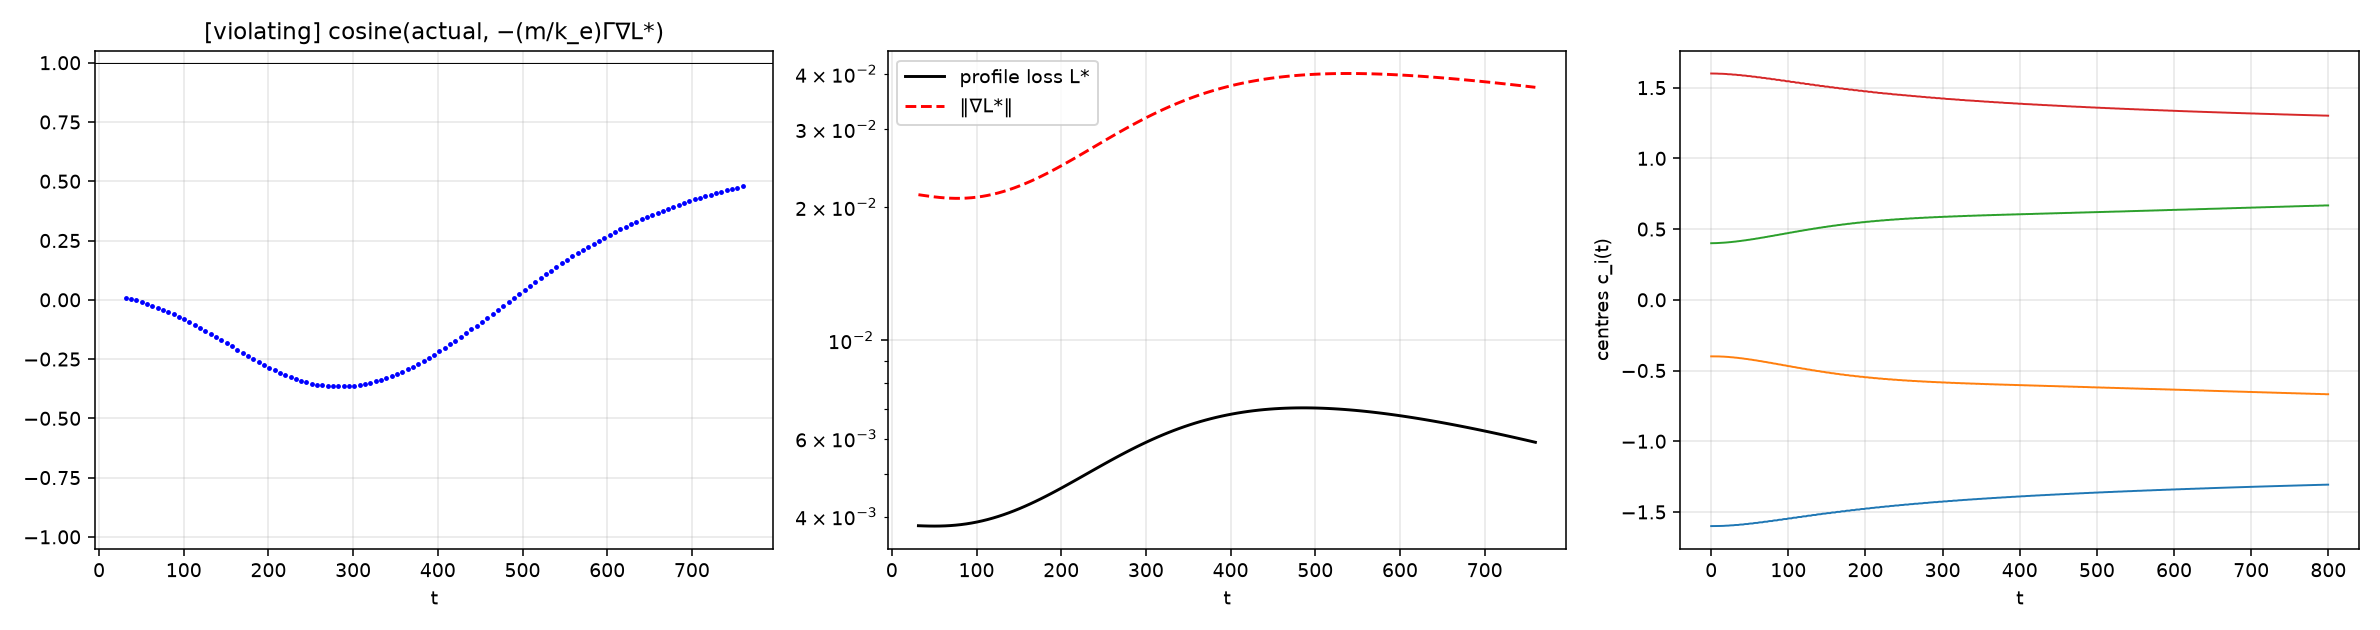
\includegraphics[width=0.95\textwidth]{variable_projection/figure_violating.png}
\caption{Proposition G, \texttt{violating} configuration. Left: the G(b) cosine between the actual geometry velocity
and the VarPro direction $-(m\delta/k_e)\Gamma\nabla L^*$, along the run. Centre: the profile loss $L^*$ and
$\norm{\nabla L^*}$. Right: the centres $c_i(t)$.}
\label{fig:evidence:violating}
\end{figure}

\begin{figure}[htbp]
\centering
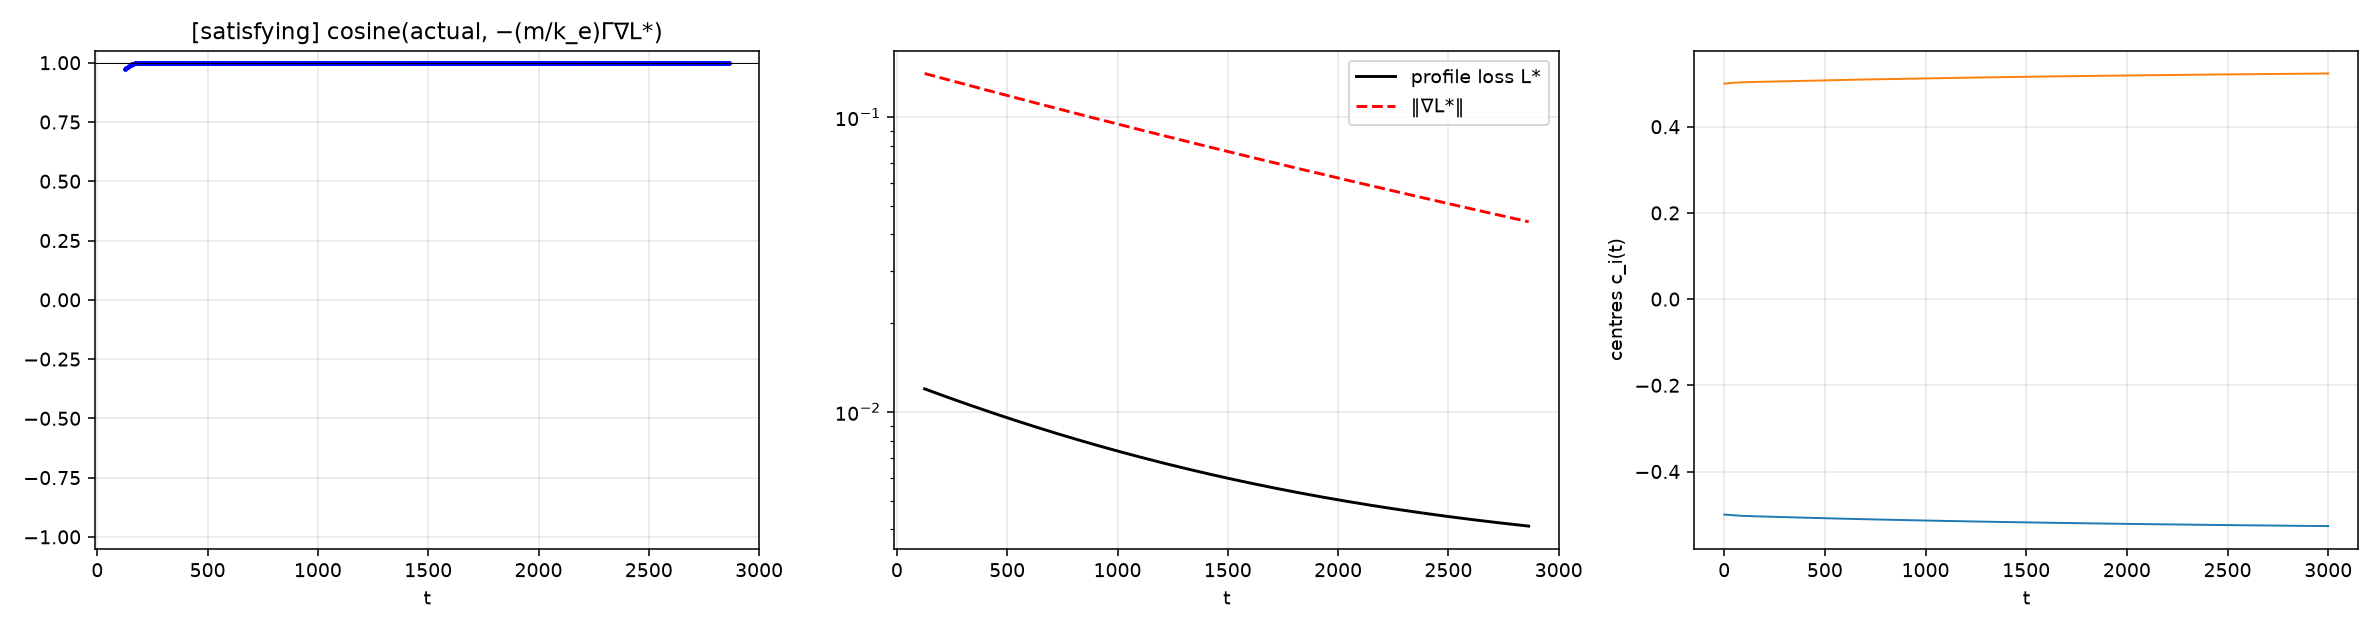
\includegraphics[width=0.95\textwidth]{variable_projection/figure_satisfying.png}
\caption{Proposition G, \texttt{satisfying} configuration; panels as in
Figure~\ref{fig:evidence:violating}.}
\label{fig:evidence:satisfying}
\end{figure}

% ------------------------------------------------------------------------------------------------ H
\subsection{Theorem H: Langevin adaptive control}

\begin{sloppypar}
\noindent Scripts: \code{exp_langevin_global.py} $\to$ \code{langevin_global/}, \code{exp_langevin_tradeoff.py}
$\to$ \code{langevin_tradeoff/}, and \code{exp_gibbs_reference.py} $\to$
\code{langevin_global/gibbs_reference.md}.
\end{sloppypar}

The setting is the real closed loop with $m=32$, a scalar plant and a periodic reference.
\begin{itemize}
  \item The unregularised offline optimum of the occupation loss is about $7.6\cdot10^{-6}$ (best of 5 L-BFGS
    restarts, an upper bound). One run gave $7.0\cdot10^{-6}$, because of floating-point summation order.
  \item \begin{sloppypar}The regularised optimum $\bar L(\mu^*_\tau)$ is $0.11118$ at $(\sigma,\tau)=(0.02,0.004)$
    and $0.00850$ at $(0.002,5\cdot10^{-4})$, grid-converged (\code{exp_gibbs_reference.py} $\to$
    \code{langevin_global/gibbs_reference.md}).\end{sloppypar}
  \item In the scaling $\sigma=0.2/k_e$, $\tau=0.04/k_e$ of Conjecture H.6, $\bar L(\mu^*_\tau)=0.11118$ for every
    $k_e$. The exactly averaged stationary state gives $\bar L=0.11415$, $0.11148$ and $0.11101$ at $k_e=10$, $20$
    and $40$. The $L^2(\rho)$ distance between the two learned functions is $6.81\cdot10^{-3}$,
    $1.43\cdot10^{-3}$ and $9.7\cdot10^{-4}$.
\end{itemize}

\paragraph{Speed--bias trade-off.} Table~\ref{tab:evidence:tradeoff} and Figure~\ref{fig:evidence:tradeoff}
($\sigma=0.002$, 2 seeds, \code{langevin_tradeoff/table.md}).

\begin{table}[htbp]
\centering
\small
\caption{Theorem H: speed--bias trade-off of parameter dither ($m=32$, $\sigma=0.002$, $k_e=10$, $T=1500$\,s,
2 seeds). The escape time is the first sample at which the collapsed run's loss is at most twice the spread run's
final loss (same seed); per-seed values are listed, and $\infty$ means not within the horizon. The losses are the
final values of $\bar L$.}
\label{tab:evidence:tradeoff}
\begin{tabular}{@{}lccc@{}}
\toprule
$\tau$ & escape of the collapsed start (s) & loss, collapsed & loss, spread\\
\midrule
0                    & $\infty$, $\infty$ & 0.166  & 0.00696\\
0.0005               & $\infty$, 1050     & 0.0249 & 0.0109\\
0.001                & 1480, 1005         & 0.0216 & 0.0148\\
0.002                & 1115, 800          & 0.0288 & 0.0233\\
0.004                & 970, 430           & 0.0392 & 0.0362\\
0.008                & 390, 295           & 0.0603 & 0.0653\\
annealed (hot start) & 990, 530           & 0.0317 & 0.0320\\
\bottomrule
\end{tabular}
\end{table}

\begin{itemize}
  \item \textbf{Fit.} The seed-averaged escape time fits $A+B\log(1/\tau)$ with an RMS relative residual of 0.045,
    against 0.253 for an Arrhenius fit. On the eight per-seed values both laws fit poorly (0.274 and 0.330). The
    data do not identify the escape mechanism, and the ``saddle'' reading of an earlier version of this analysis is
    withdrawn (Remark H.2).
  \item \textbf{Caveats.} The threshold grows with $\tau$, and the censored $\tau=5\cdot10^{-4}$ point is excluded
    from the fit.
  \item \textbf{Guaranteed rate.} The Holley--Stroock~\cite{hs1987} rate $2\tau\rho_\tau$ is at least
    $e^{-8401}$\,s$^{-1}$ at $(0.002,5\cdot10^{-4})$ and at least $e^{-1053}$\,s$^{-1}$ at $(0.02,0.004)$.
\end{itemize}

\begin{figure}[htbp]
\centering
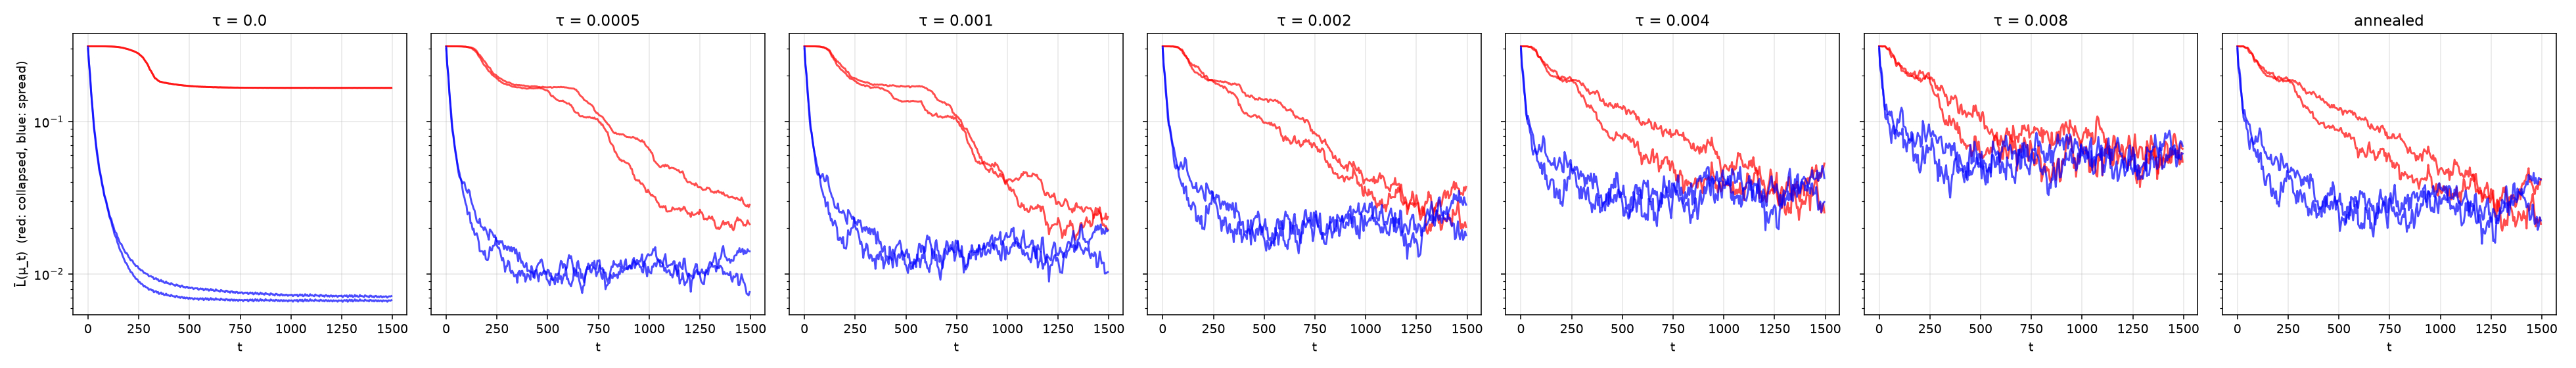
\includegraphics[width=\textwidth]{langevin_tradeoff/figure.png}
\caption{Theorem H, speed--bias trade-off: $\bar L(\mu_t)$ of the collapsed start (red) and of the spread start
(blue), 2 seeds, for $\tau=0$, $0.0005$, $0.001$, $0.002$, $0.004$, $0.008$ and the annealed (hot-start) schedule.}
\label{fig:evidence:tradeoff}
\end{figure}

\paragraph{Two fixed settings.} Three seeds (\code{langevin_global/table_*.md}; Figure~\ref{fig:evidence:global}).
\begin{itemize}
  \item \textbf{$\sigma=0.02$, $\tau=0.004$.} Both starts equalise: the loss ratio is 1.03, and the final measures
    are $4.2\times$ closer in $W$ than without dither. The common loss is about 0.11, which matches the grid value
    $\bar L(\mu^*_\tau)=0.111$. It is dominated by the regularisation bias.
  \item \textbf{$\sigma=0.002$, $\tau=5\cdot10^{-4}$.} Dither frees the collapsed start ($0.166\to0.0480$), but the
    starts do not equalise within 900\,s (loss ratio 5.23).
\end{itemize}

\begin{figure}[htbp]
\centering
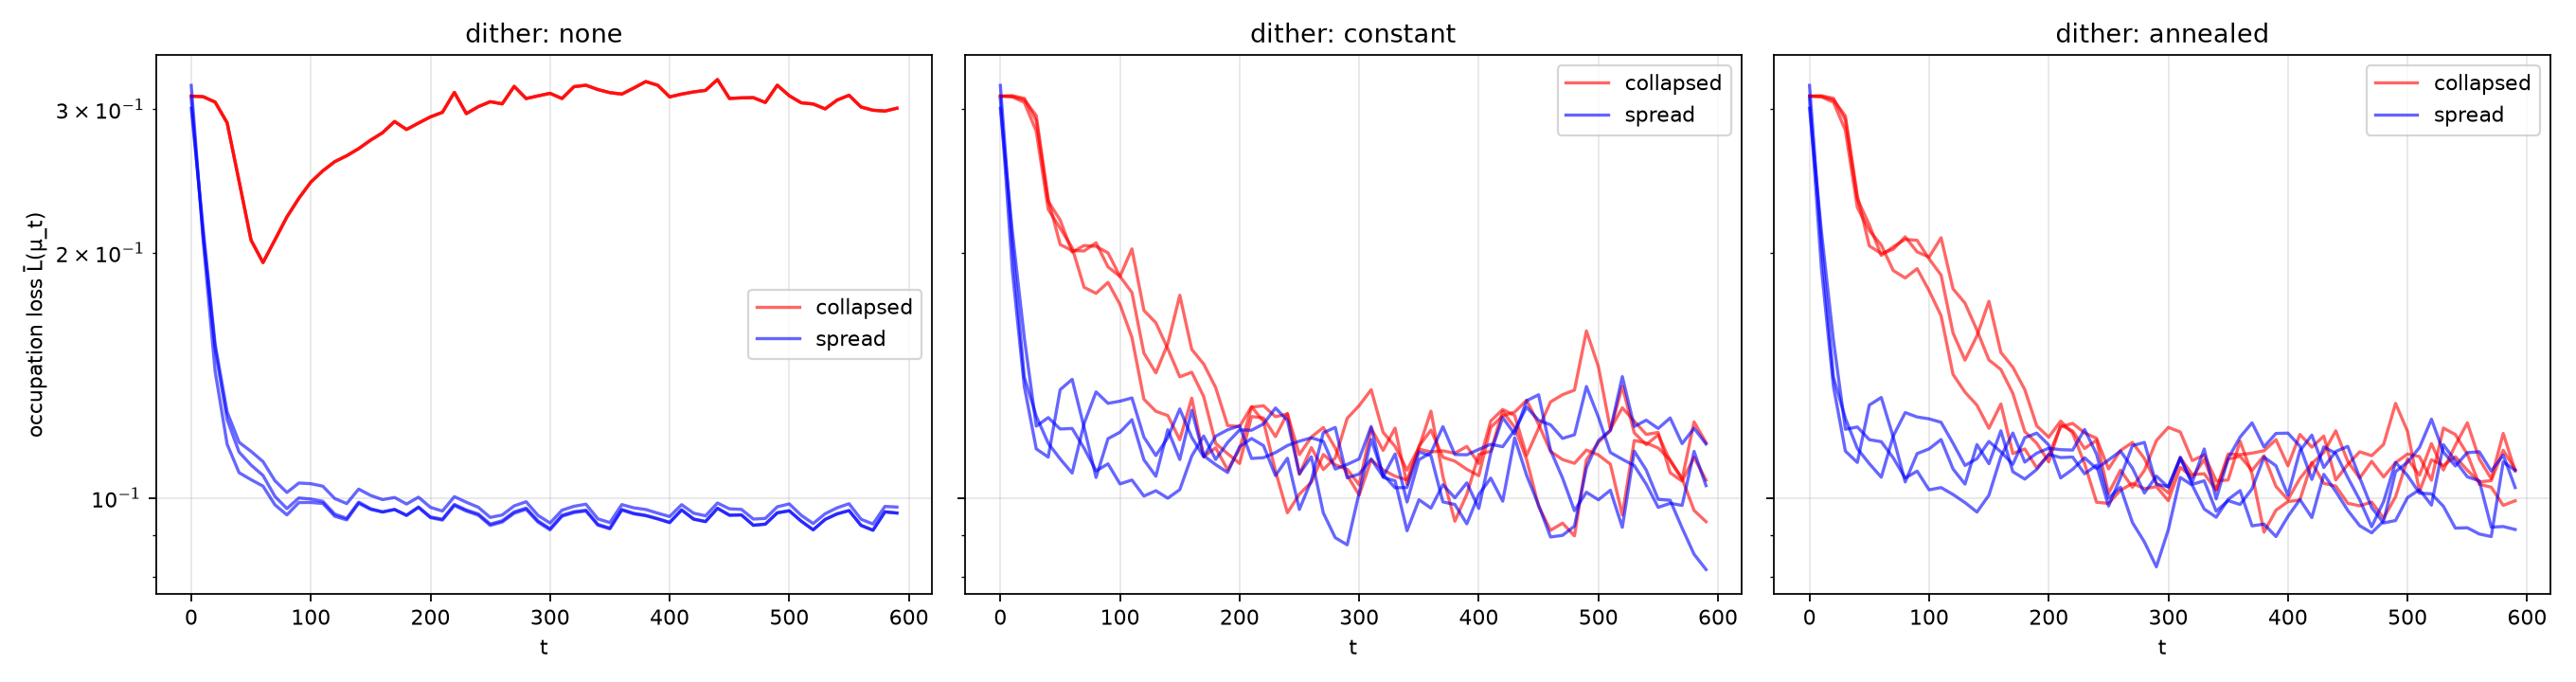
\includegraphics[width=0.95\textwidth]{langevin_global/figure_sigma0.02_tau0.004.png}\\[2pt]
{\small (a) $\sigma=0.02$, $\tau=0.004$}\\[6pt]
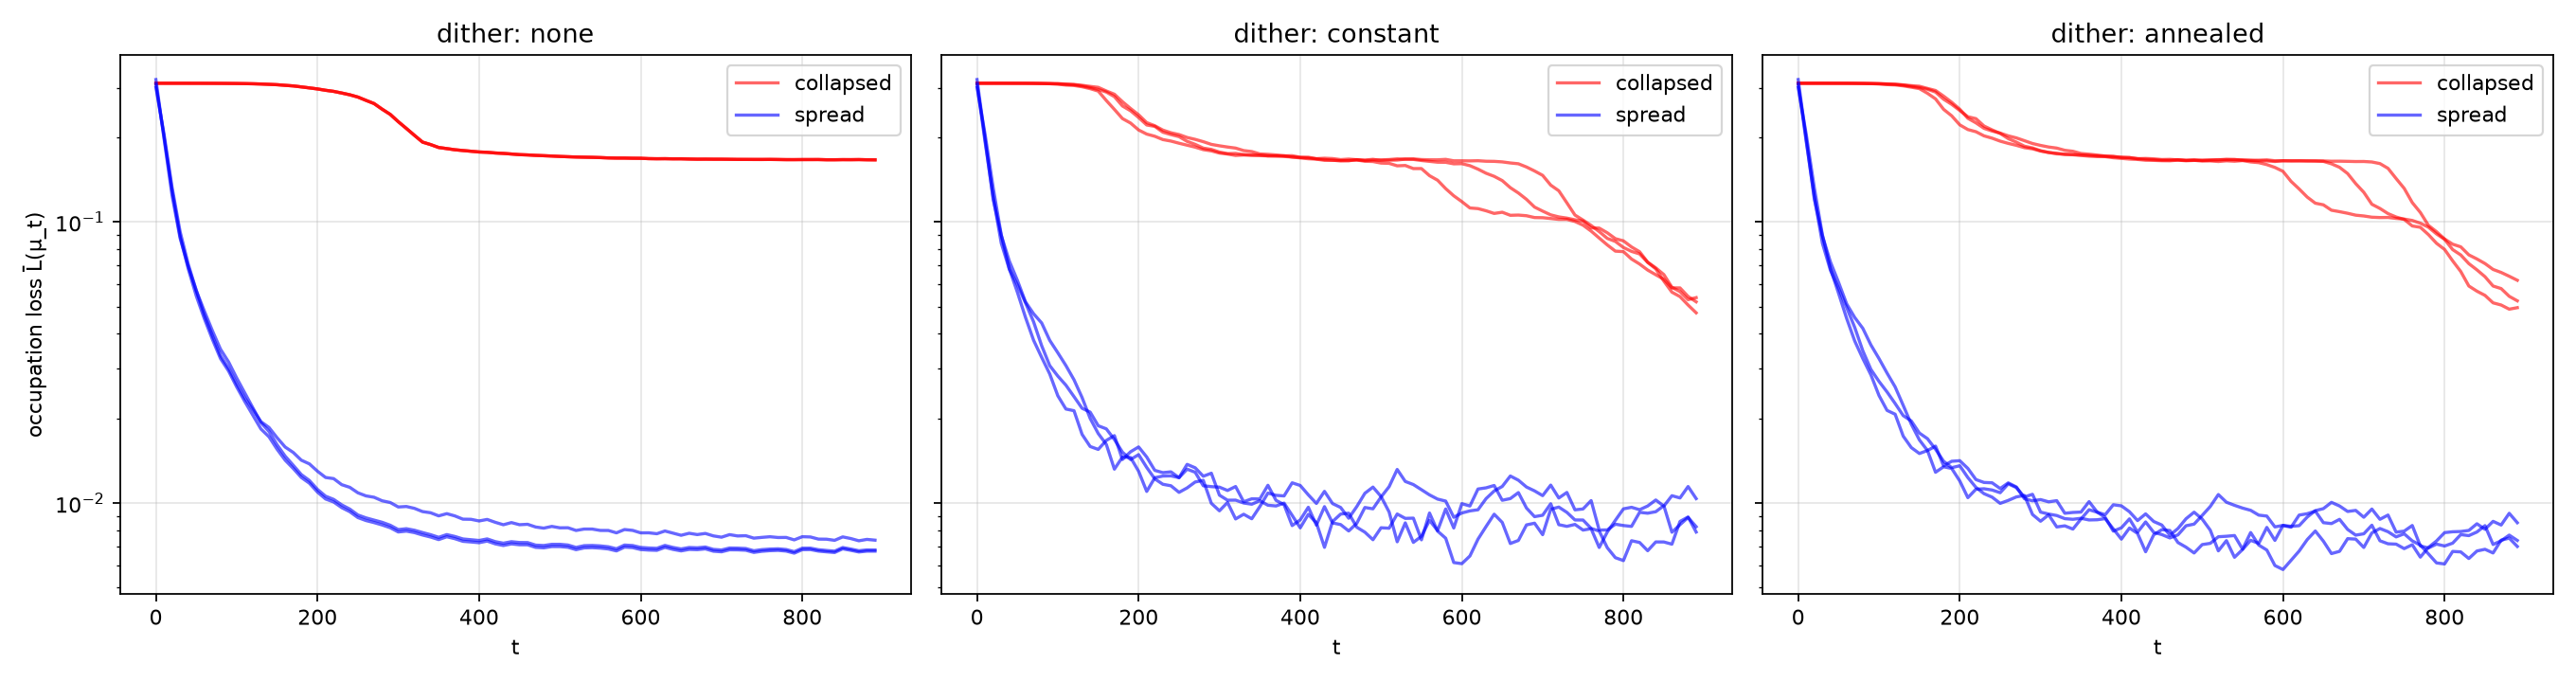
\includegraphics[width=0.95\textwidth]{langevin_global/figure_sigma0.002_tau0.0005.png}\\[2pt]
{\small (b) $\sigma=0.002$, $\tau=5\cdot10^{-4}$}
\caption{Theorem H, global kernel placement ($m=32$, scalar plant, $k_e=10$, 3 seeds): the occupation loss
$\bar L(\mu_t)$ of the collapsed and spread starts without dither, with constant dither and with annealed dither.}
\label{fig:evidence:global}
\end{figure}

% ------------------------------------------------------------------------------------------------ H.0 / H.7
\subsection{Remark H.0 and Proposition H.7: the exactly averaged closed loop}

These are checked by tests. Table~\ref{tab:evidence:averaging} gives the relative error of the frozen-$\mu$ averaged
drift against $\Aavg$, and Table~\ref{tab:evidence:structure} the structure of the first correction
(\code{test_averaging.py}).

\begin{center}
\begin{minipage}{\textwidth}
\centering
\small
\captionsetup{position=top}
\captionof{table}{Remark H.0: relative error of the frozen-$\mu$ averaged drift against $\Aavg$.}
\label{tab:evidence:averaging}
\begin{tabular}{@{}lccccc@{}}
\toprule
instance & $k_e=10$ & 20 & 40 & 80 & $k_e\times{}$error\\
\midrule
$n=1$ (\code{test_langevin.py}) & 4.2\% & 2.0\% & 0.91\% & 0.48\% & $\approx0.4$\\
$n=2$, ellipse (\code{test_averaging.py}) & 43\% & 21\% & 10\% & 5.1\% & $\approx4.2$\\
\bottomrule
\end{tabular}
\end{minipage}
\end{center}

\begin{center}
\begin{minipage}{\textwidth}
\small
\captionsetup{position=top}
\captionof{table}{Proposition H.7: structure of the first correction (\texttt{test\_averaging.py}).}
\label{tab:evidence:structure}
\begin{tabularx}{\textwidth}{@{}>{\raggedright\arraybackslash}p{0.4\textwidth}YY@{}}
\toprule
check & $n=1$ & $n=2$ (ellipse)\\
\midrule
expansion error of $k_e^2(P_\mu-P_0)$ against $U_{\mathrm{even}}+U_{\mathrm{odd}}$, $k_e=40\to80$
  & $0.54\to0.25$ & $0.038\to0.019$\\
circulation kernel $K$ & $\equiv0$ (asserted at $10^{-12}$) & antisymmetric; equals the enclosed-area integral to
  $7\cdot10^{-15}$ (asserted at $10^{-6}$)\\
orbit reversal (same $\rho$) & $U_{\mathrm{odd}}\equiv0$ & $U_{\mathrm{even}}$ unchanged, $U_{\mathrm{odd}}$
  flipped, to $2\cdot10^{-15}$ (asserted at $10^{-10}$)\\
$k_e^2\cdot{}$cyclic sum of the antisymmetric second variation, exact ($k_e=80$) against predicted (asserted at
  3\%; the full matrix at 5\%) & $-0.0711$ against $-0.0704$ & $-0.0471$ against $-0.0464$\\
\bottomrule
\end{tabularx}
\end{minipage}
\end{center}

% ------------------------------------------------------------------------------------------------ H.7a
\subsection{Remark H.7a: the orientation of the reference orbit}

Script: \code{exp_orbit_orientation.py} $\to$ \code{orbit_orientation/}.

The setup is deterministic: $n=2$, $m=6$, $G=\operatorname{diag}(4,4,1,1,1)$, $\sigma=2/k_e$, no dither. The same
elliptic reference is traversed both ways, so the occupation measure is the same, and so is the initial
configuration. The runs converged to machine precision: the residual drift over the last 10 periods is about
$10^{-16}$ (between $1.0\cdot10^{-16}$ and $5.0\cdot10^{-16}$). The six kernels converge to a common configuration
(kernel spread $1.05$ at the start, at most $5.6\cdot10^{-17}$ at the end of every run), so the learned network is
effectively a single kernel and the test probes the effect at a collapsed equilibrium. Predictions are linear responses at the $(+)$
equilibrium (Table~\ref{tab:evidence:orientation}).

\begin{table}[htbp]
\centering
\small
\caption{Remark H.7a: orientation dependence of the learned kernels in the real closed loop. Size ratios are
measured\,/\,predicted.}
\label{tab:evidence:orientation}
\begin{tabular}{@{}cccccc@{}}
\toprule
 & & \multicolumn{2}{c}{frozen-measure prediction (H.7)} & \multicolumn{2}{c@{}}{full prediction (H.7 +
  oscillation term)}\\
\cmidrule(lr){3-4}\cmidrule(l){5-6}
$k_e$ & measured $\norm{\Theta_+-\Theta_-}$ & size ratio & cosine & size ratio & cosine\\
\midrule
10 & $5.729\cdot10^{-3}$ & 2.670 & 0.7577 & 0.937 & 0.9314\\
20 & $2.843\cdot10^{-3}$ & 2.414 & 0.8302 & 0.965 & 0.9809\\
40 & $1.403\cdot10^{-3}$ & 2.294 & 0.8631 & 0.969 & 0.9944\\
\bottomrule
\end{tabular}
\end{table}

\begin{itemize}
  \item The vector error $\norm{\text{measured}-\text{predicted}}/\norm{\text{predicted}}$ of the full prediction is
    0.364, 0.195 and 0.109 at $k_e=10$, $20$ and $40$.
  \item The measured difference scales like $k_e^{-1.01}$, against a predicted $-1$.
  \item The full first-order theory accounts for it. The frozen-measure terms alone account for less than half.
  \item A first attempt with $\sigma=0.5/k_e$ and half the horizon had not converged (residual drift about a third of
    the difference). It was discarded and rerun.
\end{itemize}
